\chapter{Modello Windkessel}\label{windkessel}
In questo capitolo vengono introdotti alcuni concetti di fisiologia necessari alla comprensione del \textbf{modello Windkessel}, successivamente introdotto. Il capitolo non vuole essere completo della teoria alla base del modello, ma vuole introdurne l'idea su cui si fonda: l'\textbf{effetto Windkessel}.\\
Nel capitolo viene fatto uso di una jupyter notebook usata nel corso \textit{Introduzione a Python per il calcolo scientifico} tenuto dal professore Lucas Omar Müller nell'anno accademico 2021/2022.\\
Le fonti usate per la stesura del capitolo sono: \cite{AaronsonPhilipI.PhilipIrving2020Tcsa}, \cite{wiki:Vascularresistance}, \cite{wiki:Compliance}, \cite{wiki:WindkesselEffect},
\cite{wiki:cicloCardiaco},
\cite{wiki:DiagrammaWiggers},
\cite{westerhof_arterial_2008}, \cite{ghitti_toro_müller_2022}. \\



\begin{textblock*}{0.64\textwidth}(3.5cm+0.36\textwidth,18.5cm)
\epigraph{Medicine is a science of uncertainty and an art of probability.}{William Osler}
\end{textblock*}




\newpage

\section{Introduzione}
Da \cite{westerhof_arterial_2008} si prendono in considerazione dati di un paziente nel quale è stato misurato il flusso aortico $Q_{\text{in}}$ e la pressione sistemica $P$.

Visualizzando il grafico dei due valori si ottiene quanto in figura \ref{figDatiReali}.

\begin{figure}[h]
    \centering
    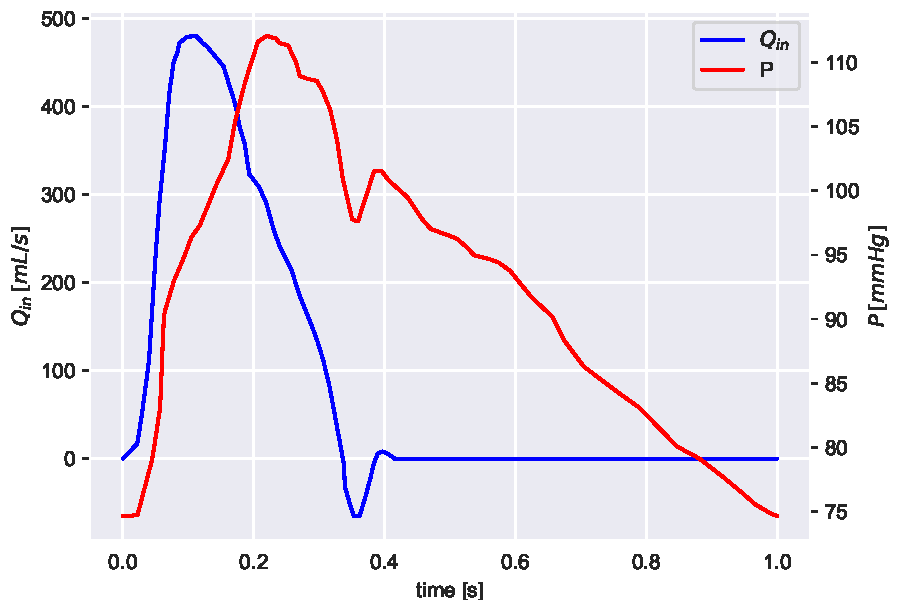
\includegraphics[width=0.7\textwidth]{images/Windkessel/DatiReali.pdf}
    \caption{Pressione sistemica e flusso aortico misurati in un paziente. Codice \ref{datiReali}.}
    \label{figDatiReali}
\end{figure}

Viene considerato ora un semplice modello del sistema cardiovascolare:
\[
P=Q_{\text{in}}R,
\]
dove $R$ è la resistenza periferica totale. Questo modello permette di calcolare la pressione arteriosa a partire dal flusso di sangue in entrata nel sistema e dalla resistenza periferica totale.



A partire dai dati reali del paziente, è possibile ricavare il valore della resistenza periferica totale $R$, o resistenza del sistema cardiovascolare. Data $T$ la durata del ciclo cardiaco, si ha:
\[
R = \frac{\frac{1}{T}\int_TP(t)dt}{\frac{1}{T}\int_TQ_{\text{in}}(t)dt}.
\]

\newpage

Ricavata $R=1.037 mmHg/mL\cdot s$ (come da codice \ref{resistenzatotale}) conoscendo $Q_{\text{in}}$ è ora possibile usare il modello per ricavare l'andamento di $P$, come mostrato in figura \ref{figModelloSemplic}.


\begin{figure}[h]
    \centering
    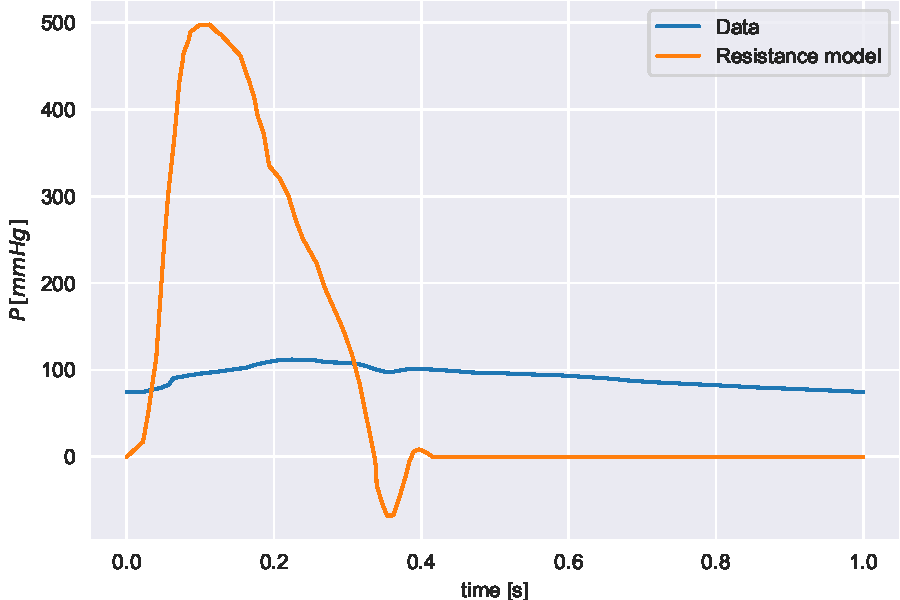
\includegraphics[width=0.7\textwidth]{images/Windkessel/modelloSemplice.pdf}
    \caption{Grafico della pressione reale e output del modello semplice. Codice \ref{modelloSemplice}.}
    \label{figModelloSemplic}
\end{figure}

Come è chiaro dalla figura, nella fase di sistole il modello prevede un picco molto alto di pressione (sull'ordine di cinque volte più alto del dato reale). Come verrà mostrato nel resto del capitolo, questo dipende dal fatto che il modello trascura un fondamentale aspetto della circolazione arteriosa: l'effetto Windkessel, cioè l'immagazzinamento di energia nelle arterie in fase di sistole.\\
A fine capitolo verrà proposto un modello che tiene conto di questo effetto e fornisce quindi un'approssimazione molto più precisa.


\newpage




\section{Concetti di fisiologia}

\subsection{Ciclo cardiaco}
Non verrà analizzato in dettaglio il ciclo cardiaco, del quale viene riportato un riassunto in tabella \ref{cicloCardiaco}, ma vengono brevemente descritti il periodo di sistole e diastole, utili alla comprensione dei prossimi argomenti. Potrà tornare utile l'immagine \ref{wiki: cuore}, in modo da avere presente l'anatomia del cuore umano necessaria alla comprensione dei successivi concetti.

\begin{figure}[h]
    \centering
    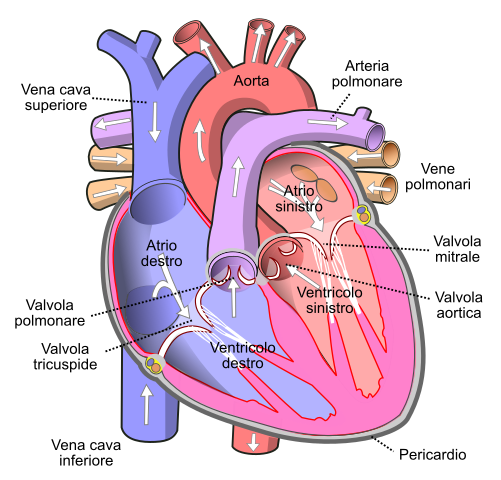
\includegraphics[width=0.7\textwidth]{images/Windkessel/Cuore.png}
    \caption{Anatomia del cuore umano \cite{wiki:cicloCardiaco}.}
    \label{wiki: cuore}
\end{figure}

La diastole cardiaca è il periodo del ciclo cardiaco in cui, dopo la contrazione, il cuore si rilassa e si espande mentre si riempie di sangue di ritorno dal sistema circolatorio. Entrambe le valvole atrioventricolari (tricuspide e mitrale) si aprono per facilitare il flusso "non pressurizzato" del sangue direttamente attraverso gli atri in entrambi i ventricoli, dove viene raccolto per la successiva contrazione. \\

La sistole atriale è la contrazione delle cellule muscolari cardiache di entrambi gli atri in seguito alla stimolazione elettrica e alla conduzione di correnti elettriche attraverso le camere atriali. \\
Definibile come parte della sequenza di contrazione ed espulsione, la sistole atriale in realtà svolge il ruolo di completare la diastole, finalizza cioè il riempimento di entrambi i ventricoli con il sangue mentre sono rilassati ed espansi per tale scopo. 

\newpage

La sistole atriale si sovrappone alla fine della diastole e applica una pressione di contrazione per spostare i volumi di sangue a entrambi i ventricoli; questo "calcio" (in inglese \textit{kick}) atriale conclude la diastole immediatamente prima che il cuore ricominci a contrarsi e ad espellere il sangue dai ventricoli (sistole ventricolare) verso l'aorta e le arterie.\\

La sistole ventricolare è la contrazione, in seguito a stimolazioni elettriche, del sincizio ventricolare di cellule muscolari cardiache nei ventricoli destro e sinistro. \\
Le contrazioni del ventricolo destro garantiscono la circolazione polmonare facendo pulsare il sangue impoverito di ossigeno attraverso la valvola polmonare e poi attraverso le arterie polmonari fino ai polmoni. Contemporaneamente, le contrazioni della sistole ventricolare sinistra forniscono la circolazione sistemica di sangue ossigenato a tutti i sistemi del corpo pompando il sangue attraverso la valvola aortica, l'aorta e tutte le arterie.\\
In figura \ref{sistoleDiastole} vengono riportati due semplici diagrammi che rappresentano lo spostamento del sangue ossigenato (rosso) e non ossigenato (blu) nelle fasi di sistole e diastole.

\begin{figure}[h]
\centering
\begin{subfigure}{0.5\textwidth}
  \centering
  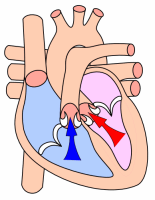
\includegraphics[width=0.5\linewidth]{images/Windkessel/sistole.png}
  \caption{Sistole}
\end{subfigure}%
\begin{subfigure}{0.5\textwidth}
  \centering
  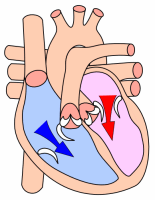
\includegraphics[width=0.5\linewidth]{images/Windkessel/diastole.png}
  \caption{Diastole}
\end{subfigure}
\caption{Diagrammi che riassumono la sistole e la diastole di un cuore umano \cite{wiki:cicloCardiaco}.}
\label{sistoleDiastole}
\end{figure}

\newpage

%%%%%%%%%%%%%%%%%%% TABELLA
\begin{landscape}
%%%%%%%%%%%%%%%%%%%%%%%%%%%%%%%%%%%%%%%%%%%%%%%
%%%%%%%%%%%%%%%%% TABELLA
%%%%%%%%%%%%%%%%%%%%%%%%%%%%%%%%%%%%%%%%%%%%%
% Please add the following required packages to your document preamble:
% \usepackage{graphicx}
\begin{table}
\centering
\resizebox{1.6\textwidth}{!}{%
\begin{tabular}{|l|c|c|l|}
\hline
\multicolumn{1}{|c|}{\textbf{Fase}} &
  \textbf{\begin{tabular}[c]{@{}c@{}}Valvole atrioventricolari\\ (tricuspide e mitrale)\end{tabular}} &
  \textbf{\begin{tabular}[c]{@{}c@{}}Valvole semilunari \\ (polmonare e aortica)\end{tabular}} &
  \multicolumn{1}{c|}{\textbf{Stato dei ventricoli e degli atri; flusso sanguigno}} \\ \hline
1 - Rilassamento isovolumetrico &
  chiuse &
  chiuse &
  \begin{tabular}[c]{@{}l@{}}Le valvole semilunari si chiudono alla fine della fase di eiezione; \\ il flusso di sangue si ferma.\end{tabular} \\ \hline
\begin{tabular}[c]{@{}l@{}}2a - Afflusso (riempimento \\ ventricolare)\end{tabular} &
  aperte &
  chiuse &
  \begin{tabular}[c]{@{}l@{}}I ventricoli e gli atri si rilassano e si espandono insieme; \\ il sangue scorre nel cuore durante la diastole ventricolare e atriale.\end{tabular} \\ \hline
\begin{tabular}[c]{@{}l@{}}2b - Influsso (Riempimento \\ ventricolare con sistole atriale)\end{tabular} &
  aperte &
  chiuse &
  \begin{tabular}[c]{@{}l@{}}Ventricoli rilassati ed espansi; la contrazione atriale (sistole) spinge \\ il sangue sotto pressione nei ventricoli durante la diastole ventricolare.\end{tabular} \\ \hline
3 - Contrazione isovolumetrica &
  chiuse &
  chiuse &
  \begin{tabular}[c]{@{}l@{}}Le valvole AV si chiudono alla fine della diastole ventricolare; \\ il flusso di sangue si ferma; i ventricoli cominciano a contrarsi.\end{tabular} \\ \hline
\begin{tabular}[c]{@{}l@{}}4 - Espulsione ventricolare\end{tabular} &
  chiuse &
  aperte &
  \begin{tabular}[c]{@{}l@{}}I ventricoli si contraggono (sistole ventricolare); il sangue scorre \\ dal cuore ai polmoni e al resto del corpo durante l'espulsione ventricolare.\end{tabular} \\ \hline
\end{tabular}%
}
\caption{Tabella riassuntiva ciclo cardiaco \cite{wiki:cicloCardiaco}.}
\label{cicloCardiaco}
\end{table}
%%%%%%%%%%%%%%%%%%%%%%%%%%%%%%%%%%%%%%%%%%%%%
%%%%%%%%%%%%%%% FINE TABELLA
%%%%%%%%%%%%%%%%%%%%%%%%%%%%%%%%%%%%%%%%%%
\end{landscape}

\newpage

Utile alla comprensione del ciclo cardiaco è il diagramma di Wiggers: è un diagramma standard che viene utilizzato nell'insegnamento della fisiologia cardiaca nel quale l'asse orizzontale viene utilizzato per tracciare il tempo mentre l'asse verticale contiene tutti i seguenti elementi su una singola griglia: pressione sanguigna, pressione aortica, pressione ventricolare, pressione atriale, volume ventricolare, elettrocardiogramma, flusso arterioso.\\
Il diagramma di Wiggers illustra chiaramente la variazione coordinata di questi valori mentre il cuore batte, aiutando a comprendere l'intero ciclo cardiaco. Aiuta anche a familiarizzare con la forma delle curve di parametri che verranno utilizzati nell'elaborato. Un esempio di diagramma viene mostrato in figura \ref{WiggersDiagramma}.


\begin{figure}[h]
    \centering
    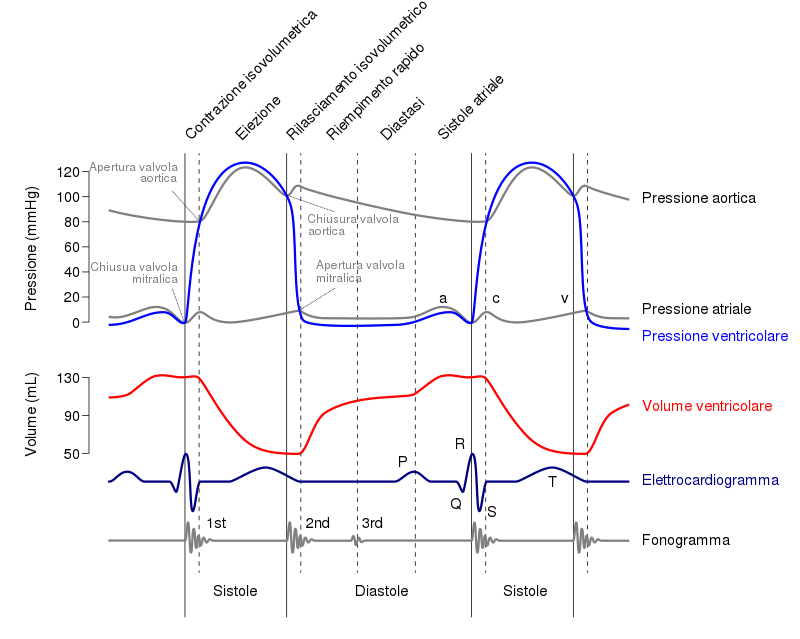
\includegraphics[width=1\textwidth]{images/Windkessel/Wiggers_Diagram_IT.svg.png}
    \caption{Esempio di diagramma di Wiggers \cite{wiki:DiagrammaWiggers}.}
    \label{WiggersDiagramma}
\end{figure}



\newpage

\subsection{Terminologia utile}\label{terminologia}

%%%%%%%%%%%%  VOLUME SISTOLIC
\subsubsection{Volume sistolico}
Il \textbf{volume sistolico} (in inglese \textit{stroke volume}, o SV) è la quantità di sangue pompato da un ventricolo ad ogni sistole ventricolare. Il volume sistolico è solitamente uguale nei due ventricoli, circa $70ml$ in un uomo sano di $70kg$.


%%%%%%%%%%%%%%%% ELASTIC ARTERY
\subsubsection{Arteria elastica}
Un'\textbf{arteria elastica} è un'arteria formata da molti filamenti di collagene ed elastina, che le conferiscono la capacità di allungarsi in risposta ad ogni pulsazione. 
\\
È proprio in virtù di questa elasticità che si ha l'effetto Windkessel, il quale aiuta a mantenere una pressione costante nelle arterie nonostante la natura pulsante del flusso sanguigno. 
\\
Le arterie elastiche comprendono le arterie più grandi del corpo, quelle più vicine al cuore.
\\
Le arterie polmonari, l'aorta e i suoi rami costituiscono insieme il sistema di arterie elastiche del corpo. Esempi sono: aorta, brachiocefalica, carotide comune, succlavia, iliaca comune.


%%%%%%%%%%%%%%% RESISTENZA VASCOLARE
\subsubsection{Resistenza vascolare}
La \textbf{resistenza vascolare} è la resistenza che deve essere superata per spingere il sangue attraverso il sistema circolatorio e creare il flusso. 
\\
La resistenza offerta dalla circolazione sistemica è nota come \textbf{resistenza vascolare sistemica} (in inglese \textit{systemic vascular resistance} o SVR) o \textbf{resistenza periferica totale} (in inglese \textit{total peripheral resistance} o TPR)\footnote{Vi è la resistenza offerta dalla circolazione polmonare nota come \textbf{resistenza vascolare polmonare}, in inglese \textit{pulmonary vascular resistance} o PVR. Non sarà però oggetto di studio in questo elaborato.}.
\\La vasocostrizione (cioè la diminuzione del diametro dei vasi sanguigni) aumenta la SVR, mentre la vasodilatazione (aumento del diametro) diminuisce la SVR.
\\
Vale la formula: $R=\frac{\Delta P}{Q}$, dove $R$ è la resistenza, $\Delta P$ la variazione di pressione durante il loop circolatorio\footnote{Cioè da subito dopo l'uscita dal ventricolo sinistro / ventricolo destro all'entrata nell'atrio destro / atrio sinistro}, $Q$ è il flusso.\\
Si noti che questa è la versione idraulica della legge di Ohm, V=IR, in cui il differenziale di pressione è analogo alla caduta di tensione elettrica, il flusso è analogo alla corrente elettrica e la resistenza vascolare è analoga alla resistenza elettrica.

\newpage
%%%%%%%%%%%%% COMPLIANCE
\subsubsection{Capacitanza o compliance}\label{capacitanza}
La \textbf{capacitanza} (o compliance, in inglese) è la capacità di un organo cavo di distendersi e aumentare di volume con l'aumento della pressione. Essa è l'equivalente fluidodinamico della capacità elettrica.\\
Nel caso dei vasi sanguigni, questo significa fisicamente che i vasi con una maggiore compliance si deformano più facilmente dei vasi con minore compliance nelle stesse condizioni di pressione e volume. \\
La compliance venosa è circa 30 volte maggiore di quella arteriosa, in gran parte a causa delle loro pareti più sottili.\\
La compliance $C$ di un vaso sanguigno è direttamente proporzionale all'elasticità delle sue pareti e costituisce una misura dei rapporti tra le variazioni di pressione e le variazioni di volume. Viene definita come: $C=\frac{\Delta V}{\Delta P}$, dove $\Delta V$ è la variazione di volume, $\Delta P$ è la variazione di pressione, cioè la differenza tra pressione intravasale e esterna.\\
Una caratteristica che rende la sua stima oggetto di studio è la difficoltà di misurazione: la compliance arteriosa può essere misurata con diverse tecniche ma la maggior parte di esse sono invasive e non sono clinicamente appropriate. 

%%%%%%%%%%%%%% EFFETTO WINDKESSEL
\subsection{Effetto Windkessel}
L'\textbf{effetto Windkessel} è un termine usato in medicina per spiegare la forma d'onda della pressione arteriosa in termini di interazione tra il volume sistolico e la compliance dell'aorta e delle grandi arterie elastiche e la resistenza delle arterie e arteriole più piccole.\\
Windkessel, dal tedesco, significa \textit{camera d'aria} e veniva usato nel diciottesimo secolo dai pompieri per garantire una continua erogazione di acqua nel combattere gli incendi; nel caso cardiovascolare si tratta di un serbatoio elastico, ma il funzionamento è lo stesso. In figura \ref{windkesselEffect} viene illustrata questa analogia.

\begin{figure}[h]
    \centering
    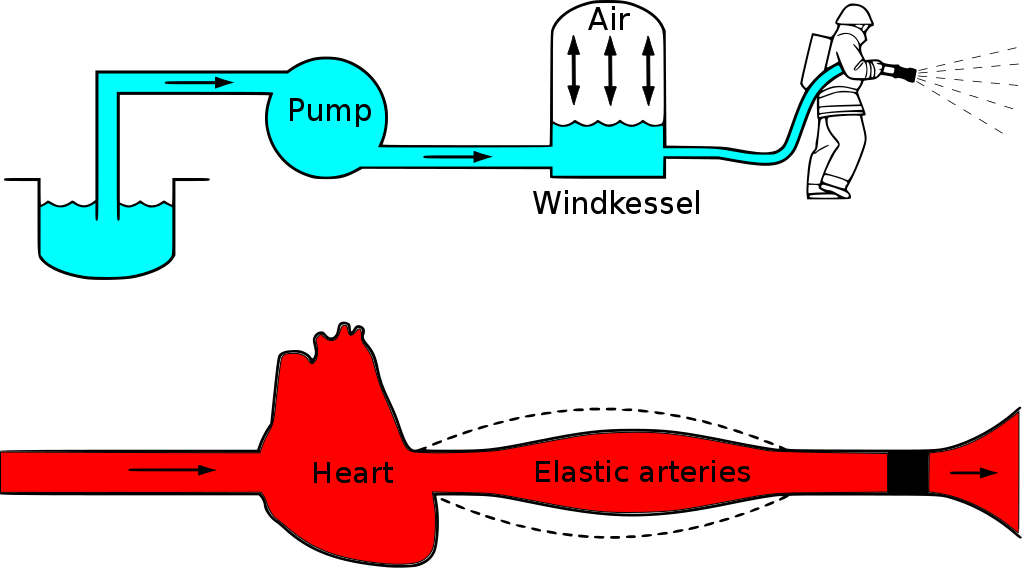
\includegraphics[width=0.7\textwidth]{images/Windkessel/WindkesselEffect.png}
    \caption{Illustrazione dell'analogia sull'effetto windkessel \cite{wiki:WindkesselEffect}.}
    \label{windkesselEffect}
\end{figure}

\newpage
Come introdotto precedentemente, le arterie elastiche si distendono quando la pressione sanguigna sale durante la sistole e si ritraggono quando la pressione sanguigna scende durante la diastole, come mostrato in figura \ref{windkesselEffect(libro)}. \\
Poiché il tasso di sangue che entra in questo tipo di arterie supera il tasso di sangue che esce, c'è un deposito netto di sangue durante la sistole, che si scarica durante la diastole. La compliance dell'aorta e delle grandi arterie elastiche è quindi analoga a quella di un condensatore; in altre parole, queste arterie agiscono collettivamente come un accumulatore idraulico.\\
L'effetto Windkessel aiuta a smorzare la fluttuazione della pressione sanguigna durante il ciclo cardiaco e aiuta a mantenere la perfusione degli organi durante la diastole, quando l'espulsione cardiaca cessa. 


\begin{figure}[h]
    \centering
    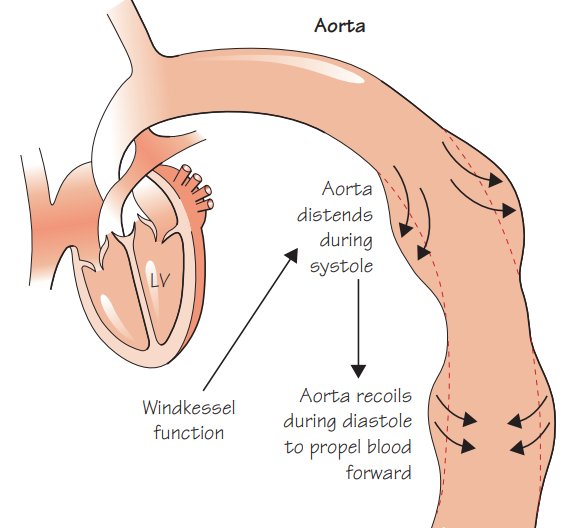
\includegraphics[width=0.7\textwidth]{images/Windkessel/WindkesselEffect(libro).PNG}
    \caption{Illustrazione dell'effetto windkessel  \cite{AaronsonPhilipI.PhilipIrving2020Tcsa}.}
    \label{windkesselEffect(libro)}
\end{figure}

\newpage

\section{Modello Windkessel a due elementi}
Nel corso dei secoli il sistema arterioso è stato modellato in molti modi e con diverse strategie. Un esempio è stato mostrato nell'introduzione a questo capitolo.
Stephen Hales\footnote{Stephen Hales (1677-1761) è stato un ecclesiastico inglese che ha dato importanti contributi ad una serie di campi scientifici tra cui la botanica, la chimica pneumatica e la fisiologia.}  fu il primo a misurare la pressione sanguigna e
notò che la pressione nel sistema arterioso non è costante,
ma varia nel corso del battito cardiaco, suggerendo che
le variazioni di pressione potessero essere legate all'elasticità delle  grandi arterie. \\
Fu Otto Frank\footnote{Otto Frank (1865 - 1944) è stato un medico e fisiologo tedesco che ha contribuito alla fisiologia cardiaca e alla cardiologia.} che formulò quantitativamente e rese popolare il cosiddetto \textbf{modello Windkessel a due elementi}
composto da un elemento di resistenza e uno di compliance.


La legge di Poiseuille afferma che la resistenza è inversamente proporzionale al raggio del vaso sanguigno alla quarta potenza. La
resistenza al flusso nel sistema arterioso è quindi principalmente
nei vasi di resistenza: le arterie più piccole e le
arteriole. Quando tutte le resistenze individuali nella microcircolazione vengono sommate correttamente, si ottiene la resistenza dell'intero
letto vascolare sistemico chiamata 
resistenza periferica (totale). La resistenza periferica, R, può
essere calcolata come:

\begin{equation}\label{R}
R = \frac{ P_{\text{ao; mean}}-P_{\text{ven; mean}}}{CO}\approx \frac{ P_{\text{ao; mean}}}{CO},
\end{equation}

dove $P_{\text{ao; mean}}$ è la pressione aortica media, mentre $P_{\text{ven; mean}}$ è la pressione venosa media, $CO$ è l'output cardiaco.\\
La componente di compliance è principalmente
determinata dall'elasticità delle grandi
arterie. Può essere ottenuta sommando le compliance
di tutti i vasi e viene quindi chiamata compliance arteriosa totale.\\
Per il calcolo di $C$ (come mostrato in \ref{capacitanza}) è molto difficile eseguire un esperimento in cui un volume viene iniettato nel sistema arterioso senza alcuna perdita nella periferia. Per questo motivo sono stati sviluppati diversi metodi per ricavare la compliance arteriosa totale senza ricorrere a esperimenti.\\
Il Windkessel a due elementi prevede che in diastole,
quando la valvola aortica è chiusa, la pressione decada
esponenzialmente con un tempo di decadimento caratteristico, con il quale è possibile calcolare la resistenza periferica con la pressione aortica in diastole e una stima della compliance arteriosa totale.\\
Il flusso medio, cioè l'output cardiaco $CO$, si ricava quindi da (\ref{R}). \\
Il Windkessel è un cosiddetto \textit{lumped} model. In altre parole, questo modello descrive l'intero sistema arterioso
in termini di una relazione pressione-flusso al suo ingresso,
sfruttando due parametri che hanno un significato fisiologico.\\
È interessante notare che in passato la ricerca si è concentrata principalmente sulla resistenza periferica, mentre il contributo della compliance arteriosa totale è stato spesso trascurato. 


Il modello Windkessel a due elementi mostra come il carico sul cuore consiste di resistenza periferica e totale arteriosa e che entrambi svolgono un ruolo importante.\\

Con lo sviluppo del flussometro elettromagnetico e quindi della misurazione del flusso aortico, è diventato chiaro che in sistole la relazione tra pressione e flusso era mal predetta dal modello Windkessel a due elementi. Le misurazioni del flusso aortico e gli sviluppi delle possibilità tecnologiche hanno portato a migliorie del modello a due elementi: il modello a tre elementi tiene conto anche della resistenza della valvola aortica, mentre il modello a quattro elementi tiene conto anche dell'inerzia del flusso sanguigno.\\

\vspace{1cm}
Per mostrare la precisione che può garantire il modello Windkessel a due elementi, viene mostrata a seguire la procedura in Python per ottenere la stima della pressione confrontandola con gli stessi dati reali usati nella sezione introduttiva.\\
Per il codice Python mostrato è necessario importare le giuste librerie mostrate nel codice \ref{configurazione1}; è necessario anche il codice \ref{flusso} che definisce la funzione di flusso\footnote{Il codice usa i dati reali ripresi da \cite{westerhof_arterial_2008}, pertanto è necessario il codice $\ref{datiReali}$.}.


\newpage

\subsection{Definizione del modello}
Come chiarito nelle definizioni in \ref{terminologia}, il modello Windkessel può essere espresso in forma di circuito come in figura \ref{circuito}.

\vspace{1cm}

\begin{figure}[h]
    \centering
    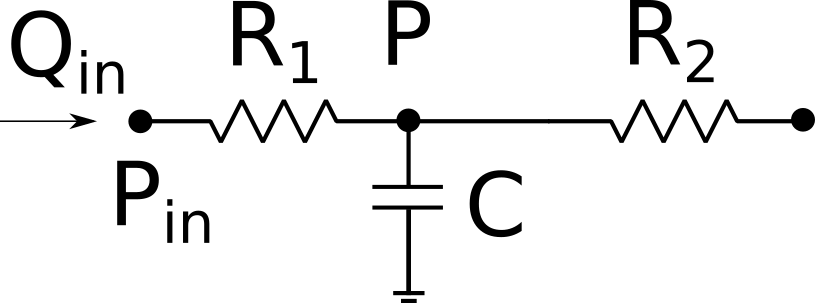
\includegraphics[width=0.6\textwidth]{images/Windkessel/Windkessel2Element.png}
    \caption{Forma circuitale del modello Windkessel a due elementi.}
    \label{circuito}
\end{figure}

Il modello Windkessel a due elementi si caratterizza dall'equazione:
\[
\frac{dP}{dt}=\frac{1}{C}(Q_{in}-Q_{out}),
\]
dove $C$ è la compliance sistemica, $R_1$ e $R_2$ sono la resistenza prossimale e periferica (di tute le arterie e arteriole), $Q_{out}$ il flusso in uscita dal capacitatore.\\
Consideriamo anche $Q_{out}=\frac{P-P_d}{R_2}$, dove $P_d$ è la pressione distale (successiva cioè alla resistenza periferica, nel corso dell'elaborato, quando non specificato altrimenti, viene imposta a $5 mmHg$), e
\begin{equation}\label{Pin}
    P_{in}=P+R_1Q_{in},
\end{equation}
da cui possiamo quindi scrivere:
\begin{equation}\label{equation}
\frac{dP}{dt}=\frac{1}{C}\left( Q_{in}-\frac{P-P_d}{R_2}\right).
\end{equation}



\subsection{Stima della compliance}
Per lavorare con l'equazione del modello è necessario conoscere la compliance. Per farlo, si minimizza la funzione
\[
f_C(C)=\sum_{n=1}^M\left( P_{in}(t_n)-\hat{P}_{in}(t_n)\right)^2,
\]
dove $\hat{P}_{in}$ è il valore misurato di pressione in $M$ punti $t_n$ e $P_{in}$ è definita come in (\ref{Pin}) e richiede di risolvere (\ref{equation}) con condizione iniziale $P(0)=\hat{P}_{in}(t_1)$.\\
Per questo primo approccio viene assunto $R_1=0$ e $R_2=R$ dove $R$ è la resistenza periferica totale. Da (\ref{Pin}) si ricava che $P_{in}=P$.\\

\newpage

Poiché è necessario risolvere l'equazione (\ref{equation}), è necessario definirla in Python come funzione, come nel codice \ref{ODE}. Si definisce poi la funzione $f_C$ nel codice \ref{fC}. Il grafico della funzione $f_C$ è mostrato in figura \ref{plotfC}.

\begin{figure}[h]
    \centering
    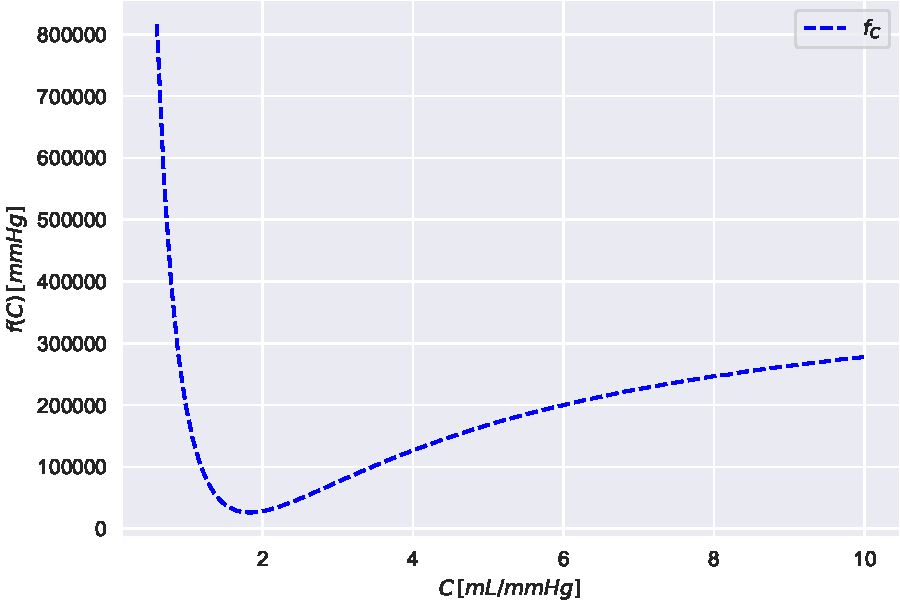
\includegraphics[width=0.75\textwidth]{images/Windkessel/f_C.pdf}
    \caption{Grafico di $f_C$. Codice \ref{plotfC-code}.}
    \label{plotfC}
\end{figure}



Dunque è ora possibile stimare $C$ che minimizza $f_C$ appoggiandosi alla libreria di Python \texttt{scipy.optimize}, come fatto nel codice \ref{stimaC}, in questo modo si trova $C=1,83288 mL/mmHg$.



Risolvendo ora l'equazione (\ref{equation}) con la $C$ stimata si ottiene quanto in figura \ref{soluzioneCapprossimata}.

\begin{figure}[h]
    \centering
    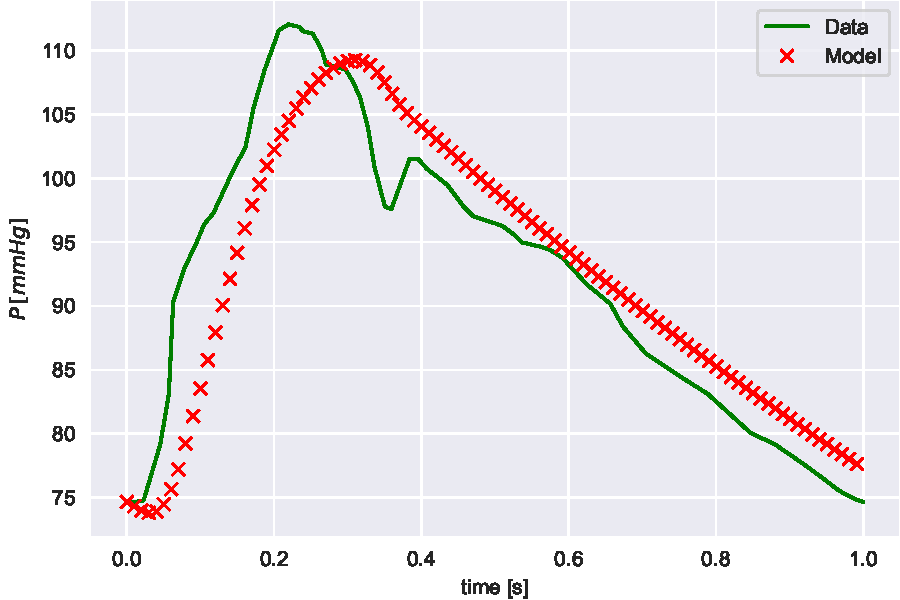
\includegraphics[width=0.75\textwidth]{images/Windkessel/modelloCstimata.pdf}
    \caption{Grafico della soluzione approssimata dell'equazione (\ref{equation}) con $C$ stimata. Codice \ref{plotSoluzioneCstimata}.}
    \label{soluzioneCapprossimata}
\end{figure}


\subsection{Stima della compliance e delle resistenze}\label{stimaCR}
Cambiando la definizione delle resistenze è possibile migliorare l'approssimazione. Si definiscono ora: $R_1=(1-\alpha)R$ e $R_2=\alpha R$ dove $\alpha\in[0,1]$. Dunque ora la funzione $f_C$ dipende anche da $\alpha$, ed è dunque necessario aggiornarla come mostrato nel codice \ref{fCa}.
Nel codice \ref{stimaCA} si stimano i parametri $C$ e $\alpha$. Si ottiene: $C=2,11579 mL/mmHg$ e $\alpha=0,97134$.
Risolvendo ora l'equazione (\ref{equation}) con i parametri stimati di $C$ e $\alpha$ si ottiene un grafico che approssima con una notevole precisione i dati reali, come mostrato in figura \ref{soluzioneCalphaapprossimata}.

\begin{figure}[h]
    \centering
    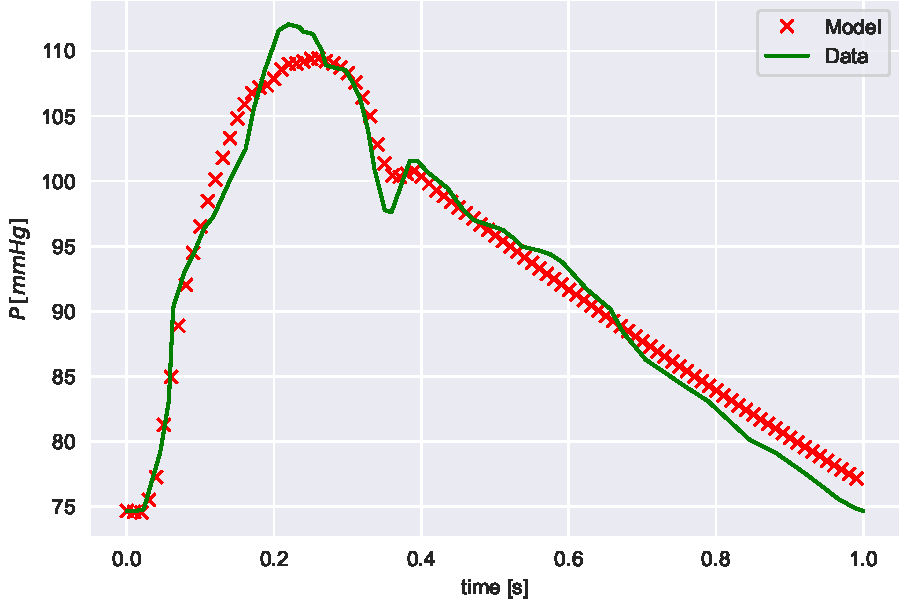
\includegraphics[width=0.75\textwidth]{images/Windkessel/modelloCalphastimata.pdf}
    \caption{Grafico della soluzione approssimata dell'equazione (\ref{equation}) con $C=2,11579mL/mmHg$ e $\alpha=0,97134$. Codice \ref{soluzioneCalphastimate}.}
    \label{soluzioneCalphaapprossimata}
\end{figure}


\section{Forzante periodica}
È un risultato noto che, dato un sistema lineare omogeneo a coefficienti costanti, cioè
\begin{equation}\label{sistema omogeneo}
    \bm{\dot{x}}(t)=A\bm{x}(t),
\end{equation}
la stabilità della soluzione esatta di tale sistema è determinata dalla parte reale degli autovalori della matrice di coefficienti $A$. In particolare, una condizione necessaria e sufficiente affinché il sistema sia asintoticamente stabile è che tutti gli autovalori di $A$ abbiano parte reale strettamente negativa. In tal caso esistono costanti positive $\alpha, \beta$ tali che
\begin{equation}\label{inequation}
||e^{At}||\leq \beta e^{-\alpha t}\quad t\geq 0.    
\end{equation}
Si dimostra ora che, quando una funzione forzante periodica $\bm{b}(t)$ viene aggiunta al sistema (\ref{sistema omogeneo}) per ottenere il
sistema disomogeneo 
\begin{equation}\label{sistema disomogeneo}
    \bm{\dot{x}}(t)=A\bm{x}(t)+\bm{b}(t),
\end{equation}
se la parte omogenea è asintoticamente stabile, allora qualsiasi soluzione del sistema non omogeneo (\ref{sistema disomogeneo}) converge a una soluzione periodica all'aumentare di $t$. La soluzione esatta del sistema disomogeneo, ottenuta con il metodo della variazione delle costanti (o metodo di Lagrange), è:
\[
\bm{x}(t)=e^{At}\bm{x}_0+e^{At}\int_0^t e^{A(t-s)}\bm{b}(s)ds
\]
dove $\bm{x}(0)=\bm{x}_0$. Data $\bm{b}(t)$ funzione forzante periodica, cioè $\bm{b}(T_0) = \bm{b}(0)$ per un certo $T_0 > 0$, è possibile ottenere una soluzione periodica del sistema disomogeneo (\ref{sistema disomogeneo}), dunque che soddisfa $\bm{x}(T_0) = \bm{x}(0)$, scegliendo opportunamente la condizione iniziale $\bm{x}_0$. Con dei semplici conti si ottiene che la suddetta condizione iniziale $\bm{x}^P_0$ per ottenere una soluzione periodica è data da
\[
\bm{x}_0^P=(I-e^{AT_0})^{-1} e^{AT_0}\int_0^{T_0} e^{-As}\bm{b}(s)ds.
\]
Si mostra ora che, a partire da una condizione iniziale diversa da $\bm{x}^P_0$, i valori della soluzione convergono ai valori della soluzione periodica all'aumentare di $t$. Sia $\bm{x}^P$ la soluzione periodica corrispondente alla condizione iniziale $\bm{x}^P_0$, sia  $\bm{x}^{NP}$ qualsiasi soluzione del sistema disomogeneo associata a una qualche condizione iniziale $\bm{x}_0^{NP}$. Allora, calcolando la norma della differenza tra le due soluzioni e applicando la (\ref{inequation}), si ottiene
\[
||\bm{x}^P(t)-\bm{x}^{NP}(t)||=||e^{At}(\bm{x}_0^P-\bm{x}_0^{NP})||\leq \beta e^{-\alpha t} ||\bm{x}_0^P-\bm{x}_0^{NP}||,
\]
nella quale $\beta e^{-\alpha t}\rightarrow 0$ per $t\rightarrow +\infty$, cioè quanto si voleva dimostrare. 

Quindi se la funzione forzante $\bm{b}(t)$ è periodica e se la parte omogenea del sistema è asintoticamente stabile, allora la soluzione esatta del problema disomogeneo convergerà alla soluzione periodica del sistema disomogeneo stesso al crescere di $t$ per qualsiasi scelta ammissibile della condizione iniziale.

\subsection{Applicazione al modello Windkessel}
Nel modello Windkessel la forzante periodica è il flusso cardiaco, come si osserva nell'equazione (\ref{equation}). Dunque, a seguito di quanto detto, invece di trovare un'approssimazione della soluzione usando il flusso di un singolo ciclo cardiaco, si trova un'approssimazione su più cicli fino a che la soluzione è, a meno di una tolleranza, uguale a quella precedente.

Per farlo è sufficiente sostituire il codice della funzione flusso \ref{flusso} con \ref{flusso periodico} e quando si risolve l'equazione differenziale sostituire \verb|t_span| e di \verb|t_eval| con \verb|t_span = [time[0],numCicli+time[-1]]| e \verb|t_eval = numCicli+time| dove \verb|numCicli| è il numero di cicli cardiaci rispetto ai quali risolvere l'equazione differenziale. 

\newpage

Con queste modifiche al codice si ripete quanto visto precedentemente per l'approssimazione di $\alpha$ e $C$ e si trova: $C=2.03424$ e $\alpha= 0.97354$. L'approssimazione della soluzione dopo venti cicli cardiaci con questi parametri viene mostrata in figura \ref{soluzionePeriodicaCalphaapprossimata}.


\begin{figure}[h]
    \centering
    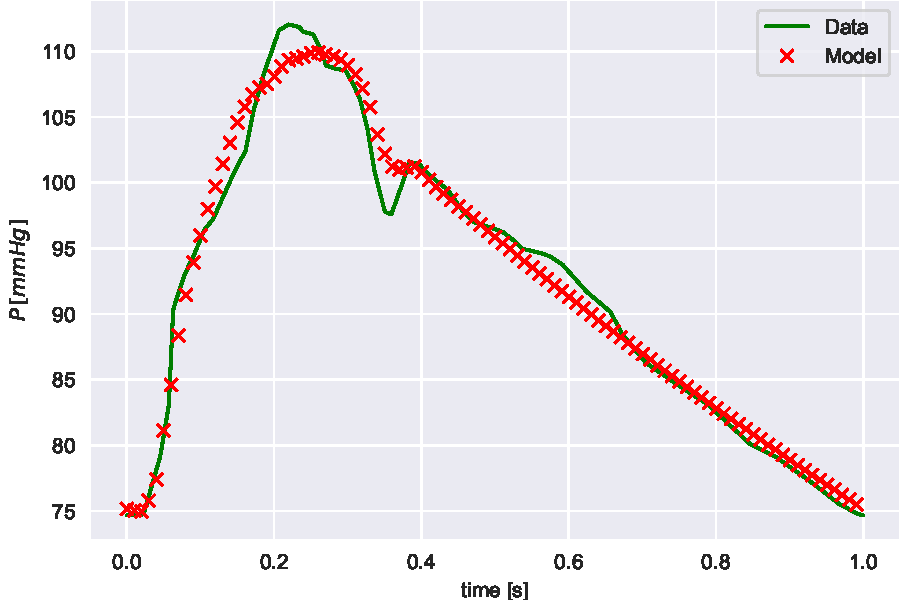
\includegraphics[width=0.75\textwidth]{images/Windkessel/modelloPeriodicoCalphastimata.pdf}
    \caption{Grafico della soluzione dell'equazione (\ref{equation}) approssimata dopo venti cicli cardiaci  con $C=2,03424mL/mmHg$ e $\alpha=0,97354$.}
    \label{soluzionePeriodicaCalphaapprossimata}
\end{figure}

Si noti che nella figura \ref{soluzioneCalphaapprossimata} l'errore della soluzione approssimata dalla pressione reale è in norma infinito $5,005246$ e in norma due $55,584739$, mentre nella figura \ref{soluzionePeriodicaCalphaapprossimata} in norma infinito è $4,654959$ e in norma due è $46,429220$. Dunque il secondo approccio, quello che tiene conto della convergenza di ogni soluzione alla soluzione periodica, genera risultati più precisi a discapito di più cicli cardiaci da considerare.


\subsection{Tempo di esecuzione} \label{Windkessel: tempo esecuzione}
Con il comando python \verb+%%timeit -r 20+ (definito un \textit{built-in magic command} delle jupyter notebook) è possibile calcolare il tempo medio e la deviazione standard di 20 esecuzioni del codice python contenuto in una cella di una jupyter notebook. Quando si cerca l'approssimazione della soluzione a convergenza si verifica che sia abbastanza simile a quella precedente, a meno di $5\times 10^{-3}$. Come spiegato in \ref{Risultati training: dataset}, il dataset di input è costituito da 3375 combinazioni di parametri $C, R_1, R_2$, per ognuna delle quali si cerca la soluzione fino a convergenza. Su tutte le combinazioni si ottengono diversi numeri di cicli necessari per arrivare a convergenza, tutti strettamente minori di cento. 

\newpage

Per dare un'idea di quanto tempo ci impieghi questo approccio, vengono mostrate in tabella \ref{tab: tempo windkessel} la quantità di tempo necessaria a trovare la soluzione dopo diversi cicli cardiaci.

\vspace{1cm}

% Please add the following required packages to your document preamble:
% \usepackage{lscape}

\begin{table}[!htb]
\centering
\begin{tabular}{cc}
\hline
\textbf{Cardiac cycles} & \textbf{\begin{tabular}[c]{@{}c@{}}Running time \\ (mean + dev. std.)\end{tabular}} \\ \hline
1   & 17.1 ms + 1.23 ms \\
10  & 90.4 ms ± 3.75 ms \\
20  & 189 ms ± 10.3 ms  \\
30  & 270 ms ± 12.9 ms  \\
40  & 362 ms ± 13.3 ms  \\
50  & 458 ms ± 15.1 ms  \\
60  & 526 ms ± 21.7 ms  \\
70  & 602 ms ± 15.9 ms  \\
80  & 711 ms ± 17.3 ms  \\
90  & 802 ms ± 32.3 ms  \\
100 & 883 ms ± 17.6 ms  \\ \hline
\end{tabular}
\caption{Run time to find the approximation of the solution of the Windkessel model over several cardiac cycles. }
\label{tab: tempo windkessel}
\end{table}





%%%%%%%%%%%%%%%%%%%%%%%%%%%%%%%%%%
%%%%%%%%% ANALISI SENSITIVITA'
%%%%%%%%%%%%%%%%%%%%%%%%%%%%%%%%
\section{Analisi di sensitività locale}\label{sensitività}
In questa sezione viene indagata la sensitività dell'output del modello ai cambiamenti dei parametri eseguendo un'\textit{analisi di sensitività locale}. \\
L'output del modello (la pressione $P$) viene utilizzato per il calcolo di quattro variabili:
\begin{itemize}
  \item $\text{MAP}$: Mean Arterial Pressure, ovvero pressione arteriosa media, si calcola come $\text{mean}(P)$;
  \item $\text{DBP}$: Diastolic Blood Pressure, ovvero la pressione sanguigna in diastole, si calcola come $\text{min}(P)$;
  \item $\text{SBP}$: Systolic Blood Pressure, ovvero la pressione sanguigna in sistole, si calcola come $\text{max}(P)$;
  \item $\text{PP}$: Pulse Pressure, ovvero la pressione di pulsazione, si calcola come $\text{max}(P)-\text{min}(P)$.
\end{itemize}

\newpage

A partire dall'output ottenuto con i valori di $C$ e $\alpha$ stimati nel codice \ref{stimaCA}, vengono riportati i valori delle variabili confrontandoli con i valori reali (di individui sani) nella tabella \ref{tab:variabili}.

% Please add the following required packages to your document preamble:
% \usepackage{graphicx}
\begin{table}[!htb]
\centering
\resizebox{0.7\textwidth}{!}{%
\begin{tabular}{cccc}
\hline
\textbf{Variables} & \textbf{Unit of measurement} & \textbf{Model} & \textbf{Real} \\ \hline
MAP                & mmHg                  & 92.91            & 65 - 110       \\
DBP                & mmHg                  & 74.86            & \textless 80   \\
SBP                & mmHg                  & 109.78           & \textless 120  \\
PP                 & mmHg                  & 34.91            & $\sim$ 40       \\ \hline
\end{tabular}%
}
\caption{Variable values calculated with the Windkessel model and input parameters ($C, \alpha$) estimated. Actual values are taken from \cite{AaronsonPhilipI.PhilipIrving2020Tcsa}.}
\label{tab:variabili}
\end{table}

Il concetto di sensitività locale è formalizzato come
\[
S_\mathcal{M}^\mathcal{P}=\frac{\hat{\mathcal{P}}}{\hat{\mathcal{M}}} \frac{\partial \mathcal{M}(\mathcal{P})}{\partial \mathcal{P}},
\]
in cui $S_\mathcal{M}^\mathcal{P}$ è la sensitività della variabile $\mathcal{M}$ al variare del parametro $\mathcal{P}$. I valori $\hat{\mathcal{M}}$ è il valore calcolato a partire dall'output del modello mentre $\hat{\mathcal{P}}$ è il valore impostato del parametro.\\

Per calcolare la derivata parziale si è fatto uso del \textit{metodo delle differenze finite centrate} riadattato al calcolo della sensitività locale, come mostrato nel codice \ref{differenzefinite}. Come variazione per ogni parametro si è usato il dieci percento del suo valore.

Per ogni parametro $\mathcal{P}=\{C,R_1,R_2,P_d\}$ si è quindi risolta il problema ai valori iniziali (\ref{equation}) due volte: una con il parametro aumentato del dieci percento, una con il parametro diminuito del dieci percento; gli altri parametri vengono lasciati invariati. I due output di $P$ ottenuti (insieme alla variazione del parametro) vengono poi usati nel metodo delle differenze finite centrate per l'approssimazione della derivata parziale. Infine si calcola la sensitività. \\
L'esempio nel caso $\mathcal{P}=C$ è mostrato nel codice \ref{Csensitivity}.
La tabella \ref{tab:local sensitivity} riassume i valori di sensitività ottenuti in ordine decrescente in modulo.

\input{Tabelle/tabella sensitività locale}

Nella tabella \ref{tab:VariazioneParametri-Variabili} viene illustrata la variazione delle variabili in funzione della variazione dei parametri.

\newpage

% Please add the following required packages to your document preamble:
% \usepackage{multirow}
% \usepackage{lscape}
\begin{landscape}
\begin{table}
\centering
\begin{tabular}{ccccccccccccc}
\hline
\textbf{Variables} &
  \textbf{$\text{MAP}_S$} &
  \textbf{$\text{MAP}_{+10\%}$} &
  \textbf{$\Delta_{MAP}$} &
  \textbf{$\text{DBP}_S$} &
  \multicolumn{1}{l}{\textbf{$\text{DBP}_{+10\%}$}} &
  \multicolumn{1}{l}{\textbf{$\Delta_{DBP}$}} &
  \multicolumn{1}{l}{\textbf{$\text{SBP}_S$}} &
  \multicolumn{1}{l}{\textbf{$\text{SBP}_{+10\%}$}} &
  \textbf{$\Delta_{SBP}$} &
  \textbf{$\text{PP}_S$} &
  \textbf{$\text{PP}_{+10\%}$} &
  \textbf{$\Delta_{PP}$} \\ \hline
\textbf{$C$} &
  \multirow{4}{*}{92.91} &
  91.81 &
  -1.18\% &
  \multirow{4}{*}{74.86} &
  74.92 &
  +0.08\% &
  \multirow{4}{*}{109.78} &
  107.32 &
  -2.24\% &
  \multirow{4}{*}{34.91} &
  32.40 &
  -7.19\% \\
\textbf{$R_1$} &
   &
  93.18 &
  +0.29\% &
   &
  74.91 &
  +0.07\% &
   &
  110.43 &
  +0.59\% &
   &
  35.52 &
  +1.75\% \\
\textbf{$R_2$} &
   &
  94.54 &
  +1.75\% &
   &
  74.93 &
  +0.09\% &
   &
  110.66 &
  +0.80\% &
   &
  35.73 &
  +2.35\% \\
\textbf{$P_d$} &
   &
  93.01 &
  +0.10\% &
   &
  74.86 &
  +0.00\% &
   &
  109.84 &
  +0.05\% &
   &
  34.98 &
  +0.20\% \\ \hline
\end{tabular}
\caption{Variation of variables as parameters increase by ten percent. $\mathcal{M}_S=\{\text{MAP}_S, \text{DBP}_S, \text{SBP}_S, \text{PP}_S\}$ are the variables obtained with standard (previously estimated) parameters, $\mathcal{M}_{+10\%}=\{\text{MAP}_{+10\%}, \text{DBP}_{+10\%}, \text{SBP}_{+10\%}, \text{PP}_{+10\%}\}$ are the variables obtained with individual parameters increased by ten percent, $\Delta=\{\Delta_{MAP}, \Delta_{DBP}, \Delta_{SBP}, \Delta_{PP}\}$ are the percentage changes in the subscript variable.}
\label{tab:VariazioneParametri-Variabili}
\end{table}
\end{landscape}

\newpage
Dalla tabella \ref{tab:VariazioneParametri-Variabili} si comprende che $P_d$ ha bassa influenza in tutte le variabili.\\
La sensitività locale si comporta quindi come ci si aspettava: più questa è alta (in modulo) e maggiore è la variazione percentuale (in modulo) della variabile modificando il parametro.\\
Ad esempio nel caso $\mathcal{M}=\text{MAP}$, la variazione in percentuale è più alta modificando $R_2$, seguita dalla variazione ottenuta modificando $C$, poi da quella modificando $R_1$ e $P_d$. Segue quindi lo stesso ordine della sensitività di $\text{MAP}$ (in modulo).\\
Si nota che $\text{DBP}$ dipende scarsamente da tutti i parametri.\\
Inoltre $C$ ha forte influenza nella variazione di $\text{SBP}$ e $\text{PP}$ (quest'ultima influenzata non trascurabilmente anche da $R_1$ e $R_2$).\\
Complessivamente $R_2$ ha maggiore influenza di $R_1$, seppur l'influenza di quest'ultima non sia trascurabile.\\

Si noti che per ogni parametro la variazione percentuale di ogni variabile ha segno inverso della sensibilità. Questo deriva dal metodo delle differenze finite centrate: con una modifica negativa si otterrebbe una variazione percentuale concorde con il segno della sensibilità.